% Retira espaço extra obsoleto entre as frases.
\frenchspacing 

% ----------------------------------------------------------
% ELEMENTOS PRÉ-TEXTUAIS
% ----------------------------------------------------------
% \pretextual

% ---
% Capa
% ---
%-------------------------------------------------------------------------
% Comentário adicional do PPgSI - Informações sobre a ``capa'':
%
% Esta é a ``capa'' principal/oficial do trabalho, a ser impressa apenas 
% para os casos de encadernação simples (ou seja, em ``espiral'' com 
% plástico na frente).
% 
% Não imprimir esta ``capa'' quando houver ``capa dura'' ou ``capa brochura'' 
% em que estas mesmas informações já estão presentes nela.
%
%-------------------------------------------------------------------------
\imprimircapa
% ---

% ---
% Folha de rosto
% (o * indica que haverá a ficha bibliográfica)
% ---
\imprimirfolhaderosto*
% ---

% ---
% Inserir a autorização para reprodução e ficha bibliografica
% ---

%-------------------------------------------------------------------------
% Comentário adicional do PPgSI - Informações sobre o texto da 
% ``autorização para reprodução e ficha bibliografica'':
%
% Página a ser usada apenas para Dissertação (tanto na versão original 
% quanto na versão corrigida).
%
% Solicitar a ficha catalográfica na Biblioteca da EACH. 
% Duas versões devem ser solicitadas, em dois momentos distintos: uma vez 
% para a versão original, e depois outra atualizada para a versão 
% corrigida.
%
% Atenção: esta página de ``autorização para reprodução e ficha 
% catalográfica'' deve ser impressa obrigatoriamente no verso da folha de 
% rosto.
%
% Não usar esta página para Qualificação.
%
% Substitua o arquivo ``fig_ficha_catalografica.pdf'' abaixo referenciado 
% pelo PDF elaborado pela Biblioteca
%
%-------------------------------------------------------------------------
\begin{fichacatalografica}
    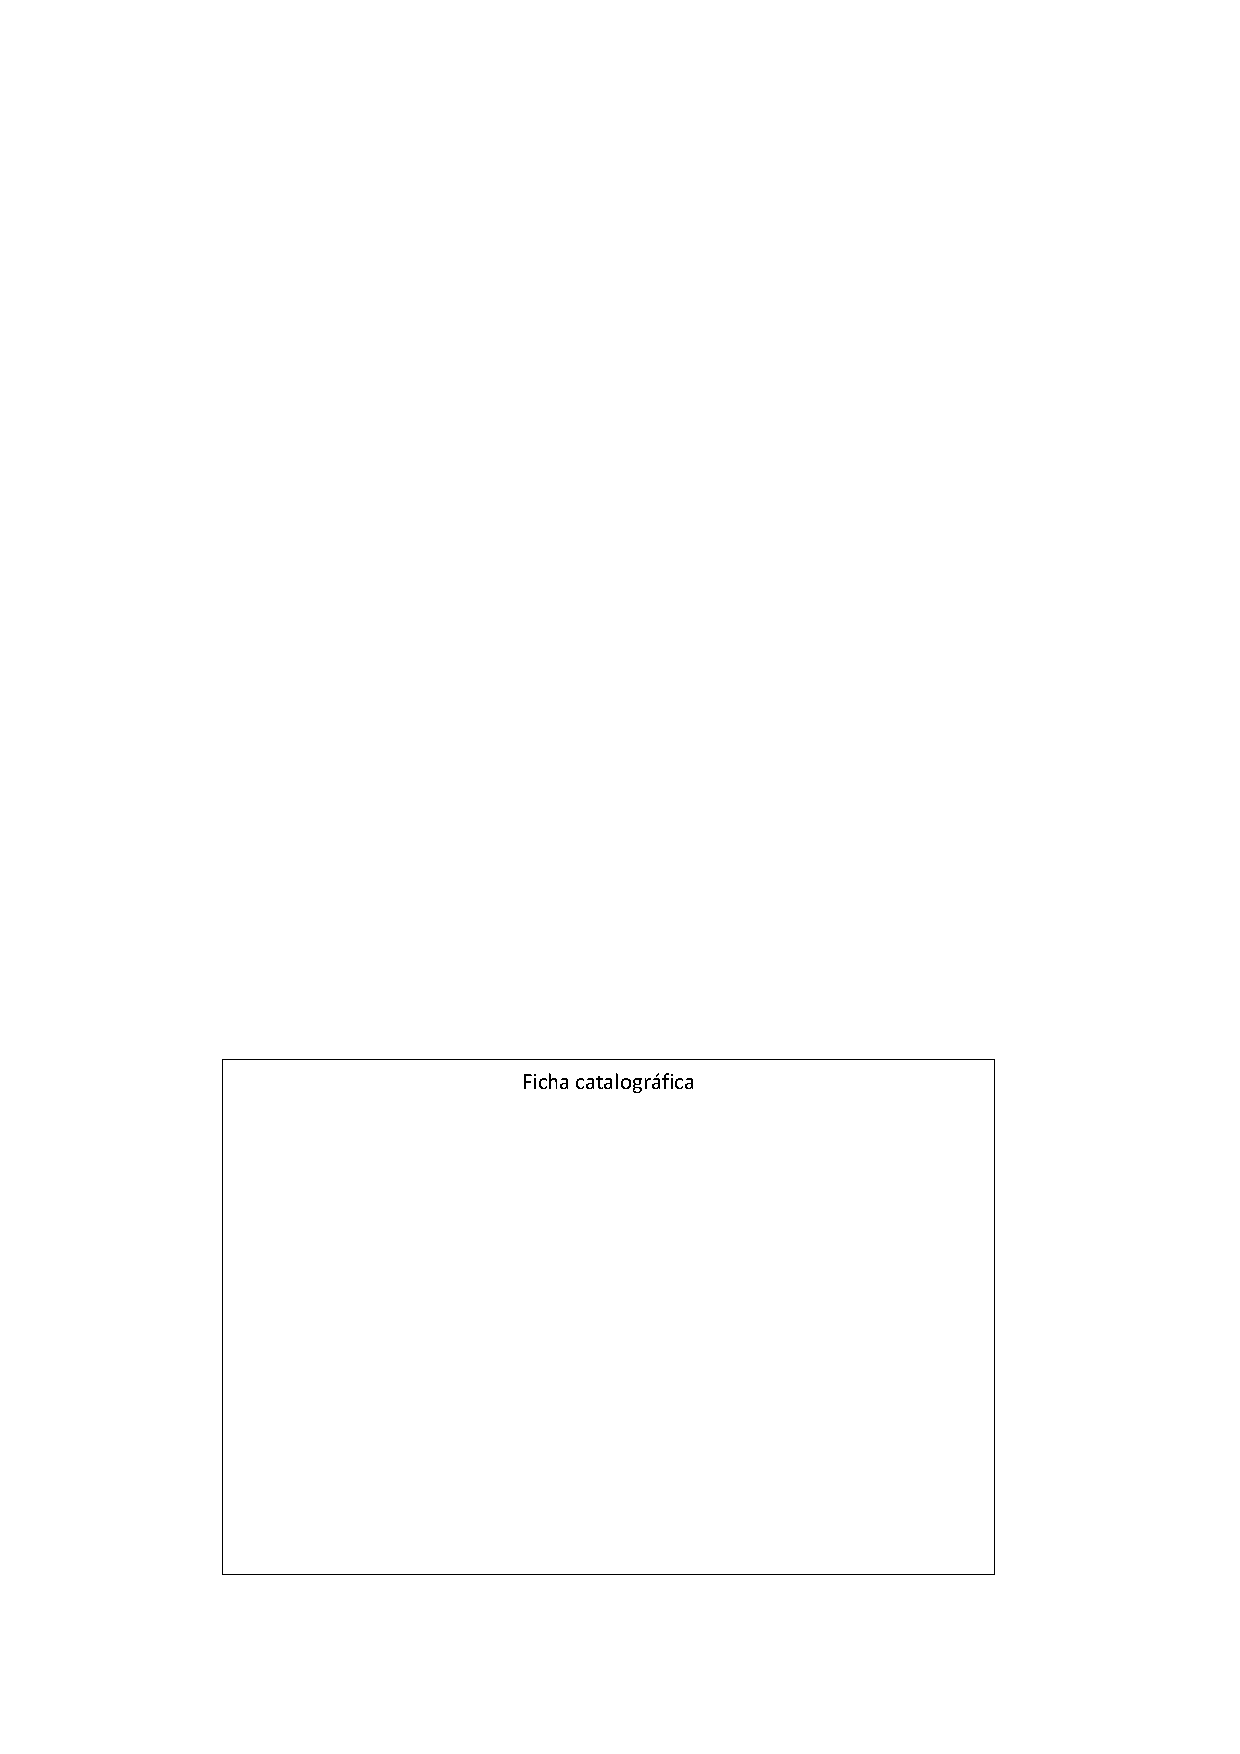
\includepdf{fig_ficha_catalografica.pdf}
\end{fichacatalografica}

% ---
% Inserir errata
% ---
%-------------------------------------------------------------------------
% Comentário adicional do PPgSI - Informações sobre ``Errata'':
%
% Usar esta página de errata apenas em casos de excepcionais, e apenas 
% para a versão corrigida da Dissertação. Por exemplo, quando depois de
% já depositada e publicada a versão corrigida, ainda assim verifica-se
% a necessidade de alguma correção adicional.
%
% Se precisar usar esta página, busque a forma correta (o modelo correto) 
% para fazê-lo, de acordo com a norma ABNT.
%
% Não usar esta página para versão original de Dissertação.
% Não usar esta página para Qualificação.
%
%-------------------------------------------------------------------------
%\begin{errata}
%Elemento opcional para versão corrigida, depois de depositada.
%\end{errata}
% ---

% ---
% Inserir folha de aprovação
% ---

\begin{folhadeaprovacao}

\noindent Dissertação de autoria de Jonas Mendonça Targino, sob o título \textbf{``\imprimirtitulo''}, apresentada à Escola de Artes, Ciências e Humanidades da Universidade de São Paulo, para obtenção do título de Mestre em Ciências pelo Programa de Pós-graduação em Sistemas de Informação, na área de concentração Metodologia e Técnicas da Computação, aprovada em \_\_\_\_\_\_\_ de \_\_\_\_\_\_\_\_\_\_\_\_\_\_\_\_\_\_\_\_\_\_ de \_\_\_\_\_\_\_\_\_\_ pela comissão julgadora constituída pelos doutores:


\vspace*{3cm}

\begin{center}
%-------------------------------------------------------------------------
% Comentário adicional do PPgSI - Informações sobre ``assinaturas'':
%
% Para Qualificação e para versão original de Dissertação: deixar em 
% branco (ou seja, assim como está abaixo), pois os membros da banca podem
% mudar, mesmo que eles já estejam previstos.
% 
% Para versão corrigida de Dissertação: usar os dados dos examinadores que 
% efetivamente participaram da defesa. 
% 
% Para versão corrigida de Dissertação: em caso de ``professora'', trocar 
% por ``Profa. Dra.'' 
% 
% Para versão corrigida de Dissertação: ao colocar os nomes dos 
% examinadores, remover o sublinhado
% 
% Para versão corrigida de Dissertação: ao colocar os nomes dos 
% examinadores, usar seus nomes completos, exatamente conforme constam em 
% seus Currículos Lattes
% 
% Para versão corrigida de Dissertação: ao colocar os nomes das 
% instituições, remover o sublinhado e remover a palavra ``Instituição:''
%
% Não abreviar os nomes das instituições.
%
%-------------------------------------------------------------------------
\_\_\_\_\_\_\_\_\_\_\_\_\_\_\_\_\_\_\_\_\_\_\_\_\_\_\_\_\_\_\_\_\_\_%\_\_\_\_\_\_\_\_\_\_\_\_\_\_\_\_\_\_\_\_\_\_
\vspace*{0.2cm} 
\\ \textbf{Prof. Dr. \_\_\_\_\_\_\_\_\_\_\_\_\_\_\_\_\_\_\_\_\_\_\_\_\_\_\_\_\_\_\_\_\_\_%\_\_\_\_\_\_\_\_\_\_\_\_\_\_\_\_\_\_\_\_\_\_\_\_\_\_\_\_
} 
\\ \vspace*{0.2cm} 
Instituição: \_\_\_\_\_\_\_\_\_\_\_\_\_\_\_\_\_\_\_\_\_\_\_\_\_\_\_\_\_\_\_\_\_\_%\_\_\_\_\_\_\_\_\_\_\_\_\_\_\_\_\_\_\_\_\_\_\_\_ 
\\ \vspace*{0.2cm}
Presidente 

\vspace*{2cm}

\_\_\_\_\_\_\_\_\_\_\_\_\_\_\_\_\_\_\_\_\_\_\_\_\_\_\_\_\_\_\_\_\_\_%\_\_\_\_\_\_\_\_\_\_\_\_\_\_\_\_\_\_\_\_\_\_
\vspace*{0.2cm} 
\\ \textbf{Prof. Dr. \_\_\_\_\_\_\_\_\_\_\_\_\_\_\_\_\_\_\_\_\_\_\_\_\_\_\_\_\_\_\_\_\_\_%\_\_\_\_\_\_\_\_\_\_\_\_\_\_\_\_\_\_\_\_\_\_\_\_\_\_\_\_
} 
\\ \vspace*{0.2cm} 
Instituição: \_\_\_\_\_\_\_\_\_\_\_\_\_\_\_\_\_\_\_\_\_\_\_\_\_\_\_\_\_\_\_\_\_\_%\_\_\_\_\_\_\_\_\_\_\_\_\_\_\_\_\_\_\_\_\_\_\_\_

\vspace*{2cm}

\_\_\_\_\_\_\_\_\_\_\_\_\_\_\_\_\_\_\_\_\_\_\_\_\_\_\_\_\_\_\_\_\_\_%\_\_\_\_\_\_\_\_\_\_\_\_\_\_\_\_\_\_\_\_\_\_
\vspace*{0.2cm} 
\\ \textbf{Prof. Dr. \_\_\_\_\_\_\_\_\_\_\_\_\_\_\_\_\_\_\_\_\_\_\_\_\_\_\_\_\_\_\_\_\_\_%\_\_\_\_\_\_\_\_\_\_\_\_\_\_\_\_\_\_\_\_\_\_\_\_\_\_\_\_
} 
\\ \vspace*{0.2cm} 
Instituição: \_\_\_\_\_\_\_\_\_\_\_\_\_\_\_\_\_\_\_\_\_\_\_\_\_\_\_\_\_\_\_\_\_\_%\_\_\_\_\_\_\_\_\_\_\_\_\_\_\_\_\_\_\_\_\_\_\_\_

\vspace*{2cm}

\_\_\_\_\_\_\_\_\_\_\_\_\_\_\_\_\_\_\_\_\_\_\_\_\_\_\_\_\_\_\_\_\_\_%\_\_\_\_\_\_\_\_\_\_\_\_\_\_\_\_\_\_\_\_\_\_
\vspace*{0.2cm} 
\\ \textbf{Prof. Dr. \_\_\_\_\_\_\_\_\_\_\_\_\_\_\_\_\_\_\_\_\_\_\_\_\_\_\_\_\_\_\_\_\_\_%\_\_\_\_\_\_\_\_\_\_\_\_\_\_\_\_\_\_\_\_\_\_\_\_\_\_\_\_
} 
\\ \vspace*{0.2cm} 
Instituição: \_\_\_\_\_\_\_\_\_\_\_\_\_\_\_\_\_\_\_\_\_\_\_\_\_\_\_\_\_\_\_\_\_\_%\_\_\_\_\_\_\_\_\_\_\_\_\_\_\_\_\_\_\_\_\_\_\_\_

\end{center}
  
\end{folhadeaprovacao}






\begin{dedicatoria}
   \vspace*{\fill}
   \centering
   \noindent
   \textit{Dedico este trabalho aos meus pais, Manoel e Josivânia, que me ensinaram que o empenho, persistência e honestidade nos levam aos mais diversos sonhos. Graças ao apoio, incentivo e paciência de minha família consigo perceber minha contribuição mediante este trabalho para com o meio científico.} 
	 \vspace*{\fill}
\end{dedicatoria}


\begin{agradecimentos} % Opcional para Dissertação.

Primeiramente, gostaria de agradecer a Deus pelo dom da vida, por ter me capacitado a vencer mais esse desafio, por sempre colocar suas mãos e me cobrir com o seu santo manto me livrando de todo o mal e me dando refúgio em momentos de angústia. Sem Deus tudo que foi feito nesta dissertação ainda estaria por fazer. 

Agradeço aos meus pais Manoel e Josivânia, por todo o apoio, incentivo e esforço que fizeram durante o desenvolvimento deste trabalho. Abdicando de inúmeras coisas para me verem onde estou hoje, pois mesmo distantes estavam torcendo pela minha vitória e me incentivando a seguir em frente, na busca de meus sonhos, por mais distantes que eles parecessem estar. Se hoje me torno uma nova pessoa é porque aprendi com meus erros, apostei em meus sonhos e em nenhum momento desisti dos mesmos.

Agradeço ao meu irmão, Vandilson e a minha tia Maria da Glória, por torcerem e rezarem pela minha vitória. Os quais se orgulham e compartilham de minhas aspirações, compartilhando comigo a satisfação de subir mais um degrau frente à ciência.

De modo especial agradeço ao meu orientador, Prof. Dr. Clodoaldo Aparecido de Moraes Lima, e a minha coorientadora, Profa. Dra. Sarajane Marques Peres pela orientação e apoio para o desenvolvimento deste trabalho de mestrado. Ambos sempre demonstraram disponibilidade para esclarecer eventuais dúvidas, fornecer sugestões e conselhos que foram essenciais para elaboração deste texto de dissertação. Com a ajuda dessa dupla consegui enxergar potenciais que nunca pensei que existiam dentro de mim.

A todos os amigos que conviveram comigo no Grupo de Inteligência Artificial (GrIA), pelo companheirismo, respeito mútuo e compartilharem inúmeras experiências e tarefas. De modo especial ao Diego Neves, Fernando Costa, Lígia Moreno, Renan Vinicius, Henrique Passos, Jozias Rolim e Jonnathann Finizola.

Agradeço também ao professor Luciano Digiampietri por dialogar comigo a respeito da vida acadêmica e por ser um exemplo de pessoa a ser seguido.

Também gostaria de agradecer ao meu amigo Josué Gomes, o qual mesmo de longe me proporciona risadas e ideias malucas que as vezes nunca saem do papel.

Por fim, e não menos importante, agradeço a CAPES pelo auxílio financeiro que permitiu com que fosse possível desenvolver este trabalho.


\end{agradecimentos}


\begin{epigrafe} % Opcional para Dissertação.
    \vspace*{\fill}
	\begin{flushright}
		%\textit{``Cada sonho que você deixa para trás, é um pedaço de seu futuro que deixa de existir''\\
		%\textit{"Ao sentir medo, por mais desconfortável que seja, sei que estou no lugar certo!"\\
		\textit{"Julgue seu sucesso pelas coisas que você teve que renunciar para conseguir"\\
		(Dalai Lama)}
	\end{flushright}
\end{epigrafe}



% resumo em português
\setlength{\absparsep}{18pt} % ajusta o espaçamento dos parágrafos do resumo
\begin{resumo}

%-------------------------------------------------------------------------
% Comentário adicional do PPgSI - Informações sobre ``referência'':
% 
% Troque os seguintes campos pelos dados de sua Dissertação (mantendo a 
% formatação e pontuação):
%   - SOBRENOME
%   - Nome1
%   - Nome2
%   - Nome3
%   - Título do trabalho: subtítulo do trabalho
%   - AnoDeDefesa
%
% Mantenha todas as demais informações exatamente como estão.
% 
% [Não usar essas informações de ``referência'' para Qualificação]
%
%-------------------------------------------------------------------------
\begin{flushleft}
Targino, Jonas Mendonça. \textbf{\imprimirtitulo}. \imprimirdata. \pageref{LastPage} f. Qualificação (Mestrado em Ciências) – Escola de Artes, Ciências e Humanidades, Universidade de São Paulo, São Paulo, 2018.
\end{flushleft}

Há um crescente incentivo ao uso da tecnologia biométrica para melhorar, e até mesmo substituir os métodos tradicionais de segurança. O campo da Biometria refere-se a uma grande variedade de tecnologias usadas para identificar ou verificar a identidade de uma pessoa por meio da mensuração e análise de vários aspectos físicos e comportamentais do ser humano. Modalidades biométricas são características extraídas do corpo humano, que são únicas para cada indivíduo e que podem ser usadas para estabelecer sua identidade numa população. As principais modalidades biométricas empregadas são: impressão digital, face, voz, palma da mão, e íris. Dentre as modalidades biométricas, a face é a mais comumente vista e usada em nossa vida diária. Em aplicações de mundo real, sistemas de reconhecimento facial, frequentemente, têm que lidar com condições não controladas e não previsíveis tais como mudança na iluminação, pose, expressão e oclusão, as quais introduzem variações intraclasse e degradam performance de reconhecimento. Comparada com problemas de pose, iluminação e expressão, o problema relacionado à oclusão é relativamente pouco estudado na área. Há dois problemas distintos relacionados com o reconhecimento facial com oclusão: detecção da face ocluída e a reconstrução da face ocluída. O objetivo desta dissertação é investigar, avaliar e comparar técnicas para detecção e reconstrução de oclusões parciais em imagens de face, obtidas em ambientes não cooperativos. Também durante a realização desse estudo comparativo foram implementadas três novas técnicas (duas baseadas em modelo e uma baseada em subespaço) de reconstrução, as quais apresentaram consideráveis taxa de reconhecimento nas bases de dados AR e Yale. Os resultados demonstram que duas das técnicas criadas nesse trabalho apresentaram consideráveis resultados de acurácia perante as técnicas dispostas na literatura.

Palavras-chaves: Detection occlusion. Occluded Face. Face reconstruction. Biometric Recognition.
\end{resumo}

% resumo em inglês
%-------------------------------------------------------------------------
% Comentário adicional do PPgSI - Informações sobre ``resumo em inglês''
% 
% Caso a Qualificação ou a Dissertação inteira seja elaborada no idioma inglês, 
% então o ``Abstract'' vem antes do ``Resumo''.
% 
%-------------------------------------------------------------------------
\begin{resumo}[Abstract]
\begin{otherlanguage*}{english}

%-------------------------------------------------------------------------
% Comentário adicional do PPgSI - Informações sobre ``referência em inglês''
% 
% Troque os seguintes campos pelos dados de sua Dissertação (mantendo a 
% formatação e pontuação):
%     - SURNAME
%     - FirstName1
%     - MiddleName1
%     - MiddleName2
%     - Work title: work subtitle
%     - DefenseYear (Ano de Defesa)
%
% Mantenha todas as demais informações exatamente como estão.
%
% [Não usar essas informações de ``referência'' para Qualificação]
%
%-------------------------------------------------------------------------
\begin{flushleft}
Targino, Jonas Mendonça. \textbf{Comparative analysis of techniques for detecting and reconstructing partial occlusions in face images for biometric recognition}. \imprimirdata. \pageref{LastPage} p. Qualification (Master of Science) – School of Arts, Sciences and Humanities, University of São Paulo, São Paulo, 2018. 
\end{flushleft}

There is a growing incentive to use biometric technology to improve, even replace, traditional security methods. The field of Biometrics refers to a wide variety of technologies used to identify or verify a person's identity by measuring and analyzing various physical and behavioral aspects of the human being. Biometric modes are characteristics drawn from the human body, which are unique to each individual and can be used to establish their identity in a population. The main biometric modalities used are: fingerprint, face, voice, palm, and iris. Among the biometric modalities, the face is the most commonly seen and used in our daily life. In real-world applications, facial recognition systems often have to deal with uncontrolled and unpredictable conditions such as change in illumination, pose, expression, and occlusion, which introduce intraclass variations and degrade recognition performance. Compared with problems of pose, illumination and expression, the problem related to occlusion is relatively little studied in the area. There are two distinct problems related to facial recognition with occlusion: detection of the occluded face and reconstruction of the occluded face. The objective of this dissertation is to investigate, evaluate and compare techniques for detection and reconstruction of partial occlusions in face images obtained in non-cooperative environments. Also during the accomplishment of this comparative study were implemented three new techniques (two based on model and one based on subspace) of reconstruction, which presented considerable recognition rate in the AR and Yale databases. The results demonstrate that two of the techniques created in this work presented considerable accuracy results in the literature.

Keywords: Detection. Occlusion. Occluded. Face. Biometric. Recognition
\end{otherlanguage*}
\end{resumo}


% ---
% ---
% inserir lista de figuras
% ---
\pdfbookmark[0]{\listfigurename}{lof}
\listoffigures*
\cleardoublepage
% ---


% ---
% ---
% inserir lista de algoritmos
% ---
\pdfbookmark[0]{\listalgorithmname}{loa}
\listofalgorithms
\cleardoublepage

% ---
% inserir lista de tabelas
% ---
\pdfbookmark[0]{\listtablename}{lot}
\listoftables*
\cleardoublepage
% ---



% ---
% inserir lista de quadros
% ---
\pdfbookmark[0]{\listofquadrosname}{loq}
\listofquadros*
\cleardoublepage
% ---
% ---
% inserir lista de abreviaturas e siglas
% ---
%-------------------------------------------------------------------------
% Comentário adicional do PPgSI - Informações sobre ``Lista de abreviaturas 
% e siglas'': 
%
% Opcional.
% Uma vez que se deseja usar, é necessário manter padrão e consistência no
% trabalho inteiro.
% Se usar: inserir em ordem alfabética.
%
%-------------------------------------------------------------------------



\begin{siglas}
  \item[APCA] \textit{Asymmetrical Principal Component Analysis}
	\item[ASM] \textit{Active Shape Model}
	\item[BMA] \textit{Block Matching Algorithm}
	\item[CNN] \textit{Convolutional Neural Network
}	\item[CST] \textit{Color Space Technique}
	\item[DCT]  \textit{Discrete Wavelet Transform}
	\item[DFFS]  \textit{Distance From face Space}
	\item[DICW] \textit{Dynamic Image to Class Warping}
	\item[ERR] \textit{Equal Error Rate}
	\item[EOH] \textit{Exceptional Occlusion  Handling}
	\item[FAR] \textit{False Acceptance Rate}
	\item[FARO] \textit{Face Recognition Against Occlusion}
	\item[FRPCA] \textit{Fast Robust Principal Component Analysis}
	\item[FRR] \textit{False Recognition Rate}
	\item[FWPCA] \textit{Fast-Weighted Principal Component Analysis}
	\item[GMM] \textit{Gaussian Mixture Models}
	\item[GPCA] \textit{Gappy Principal Component Analysis}
	\item[HMM] \textit{Hidden Markov Models}
	\item[IBD] \textit{Inpainting for Big Data}
	\item[ICP] \textit{Iterative Closest Point}
	\item[IFR] \textit{Iterative Face Recovery}
	\item[IKFDA]\textit{ Incremental Kernel Fisher Discriminant Analysis}
	\item[KAM] \textit{ Kernel Associative Memory}
	\item[KNN]  \textit{K-Nearest Neighbors}
	\item[LBP] \textit{Local binary patterns}
	\item[MCC] \textit{Matthews correlation coefficient}
	\item[MLWNN] \textit{Multi Library Wavelet Neural Network}
	\item[PCA] \textit{Principal Component Analysis}
	\item[PIN] \textit{Personal Identification Number}
	\item[PSNR] \textit{Peak Signal-to-noise Ratio}
	\item[RGEF] \textit{Reformed Gabor Eigenfaces}
	\item[RMSE] \textit{Root Mean Square Error}
	\item[ROC] \textit{Receiver Operating Characteristic}
	\item[RPCA] \textit{Robust Principal Component Analysis}
	\item[RS] Revisão Sistemática
	\item[SOM] \textit{Self Organazing Maps}
	\item[SRC] \textit{Sparse Representation Classification}
	\item[SRF] \textit{System Recognition Faces}
	\item[SSD] \textit{Sum of Square Distance}
	\item[SSEC] \textit{Structured Sparse Error Coding}
	\item[SSIM] \textit{Structural Similarity}
	\item[TLRC] \textit{Trimmed Linear Regression Classification}
	\item[UOM] \textit{Universal Occlusion Model}


    
\end{siglas}


% ---

% inserir lista de abreviaturas e siglas
% ---
%%%%% This removes the main title:%%%%%%%
%\renewcommand{\nomname}{Lista de abreviaturas e siglas}
%%%%%%% this modifies item separation: %%%%% 
%\setlength{\nomitemsep}{1.5pt}
%   \renewcommand\nomgroup[1]{%
%     \item[\Large\bfseries
%     \ifstrequal{#1}{N}{Nomenclature}{%
%     \ifstrequal{#1}{A}{List of Abbreviations}{}}%
%   ]\vspace{10pt}} % this is to add vertical space between the groups.
%
%\printnomenclature[2cm] 

% exemplos:\nomenclature[A]{\textbf{IMO}}{in my opinion}
% ---
% ---
% inserir lista de símbolos
% ---
%-------------------------------------------------------------------------
% Comentário adicional do PPgSI - Informações sobre ``Lista de símbolos'': 
%
% Opcional.
% Uma vez que se deseja usar, é necessário manter padrão e consistência no
% trabalho inteiro.
% Se usar: inserir na ordem em que aparece no texto.
% 
%-------------------------------------------------------------------------
\begin{simbolos}
\item[$\Gamma$] Conjunto de imagens de face presentes no conjunto de treinamento das técnicas de reconstrução
\item[$\Theta_i$] Vetor contendo a diferença entre a imagem de consulta e a imagem média
\item[$\Phi$] Espaço de faces
\item[$\Phi^{no}$] Espaço de faces da parte não ocluída
\item[$\Phi^{P}$] Pseudo espaço de faces
\item[$\Upsilon$] Imagem de consulta (imagem parcialmente ocluída)
\item[$\beta$] Autovetores
\item[$\beta^{no}$] Autovetores da parte não ocluída
\item[$\partial$] Derivada parcial
\item[$\mu$] Média das imagens de face presentes no conjunto de treinamento
\item[$\mu_i$] Imagem média dos indivíduos da classe \textit{i}
\item[$\alpha^{no}$] Coeficientes de combinação linear da parte não ocluída
%\item[$\phi_i$] Eigenface \textit{i} 
\item[$\kappa$] Coeficiente de multiplicação aplicado as matrizes Laplacianas
\end{simbolos}



\pdfbookmark[0]{\contentsname}{toc}
\tableofcontents* %inserir o sumário
\cleardoublepage
\textual